\section{Auswertung}
\label{sec:Auswertung}
Die direkt an der Monozelle abgegriffene Leerlaufspannung $U_\text{0}$ ergibt sich etwa zu $1.5 \si{\ohm}$.
Der Fehler des Voltmeters beträgt nach Herstellerangaben im verwendeten Messbereich $1.5\%$.
Damit ergibt sich $U_\text{0}=(1.5 \pm 0.0225) \si{\ohm}$.
Der Innenwiderstand des Voltmeters ist nach Herstellerangaben $R_\text{V}\approx 10 \cdot 10^6 \si{\ohm}$.

Der Innenwiderstand $R_\text{i}$ und die Leerlaufspannung $U_\text{0}$ der Monozelle ergeben sich mit Linearer Regression nach \eqref{eqn:ausgleichsgrade} unter Verwendung von Formel ???.
Dazu werden die in Tabelle \ref{tab:monozelle} gelisteten $U_\text{k}$ gegen $I$ aufgetragen.
\begin{equation*}
  -a= R_\text{i}=(15.5\pm0.3)\si{\ohm}
\end{equation*}
\begin{equation*}
  b =U_\text{0}=(1501.4\pm13.9)\si{\milli\volt}
\end{equation*}


\begin{table}
  \centering
  \label{tab:monozelle}
  \caption{Messdaten für die Klemmenspannung in Abhängigkeit des Strom bei der Monozelle}
\begin{tabular}{cc}
  \toprule
$U_\text{k}$/$\si{\milli\volt}$ & $I$/$\si{\milli\ampere}$\\
\midrule
69.0 & 91.0 \\
342.0 & 74.0 \\
550.0 & 61.0 \\
700.0 & 52.0 \\
825.0 & 45.0 \\
910.0 & 40.0 \\
965.0 & 37.0 \\
980.0 & 35.0 \\
990.0 & 32.0 \\
1026.0 & 30.0 \\
1056.0 & 28.0 \\
1083.0 & 26.0 \\
1110.0 & 24.0 \\
1116.0 & 23.0 \\
\bottomrule
\end{tabular}
\end{table}
\begin{figure}
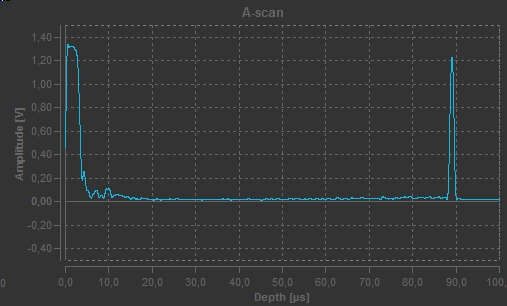
\includegraphics{Bilder/a.pdf}
\caption{Linearer Fit zur Monozelle ohne Gegenspannung}
\label{fig:plot_a}
\end{figure}
